\documentclass[tikz,border=6pt]{standalone}
\usepackage{amsmath}
\usepackage{helvet}
\usepackage{xcolor}
\renewcommand{\familydefault}{\sfdefault}
\usetikzlibrary{arrows.meta,calc}

\definecolor{myblue}{HTML}{377EB8}
\definecolor{myred}{HTML}{E41A1C}
\definecolor{myviolet}{HTML}{984EA3}

\begin{document}

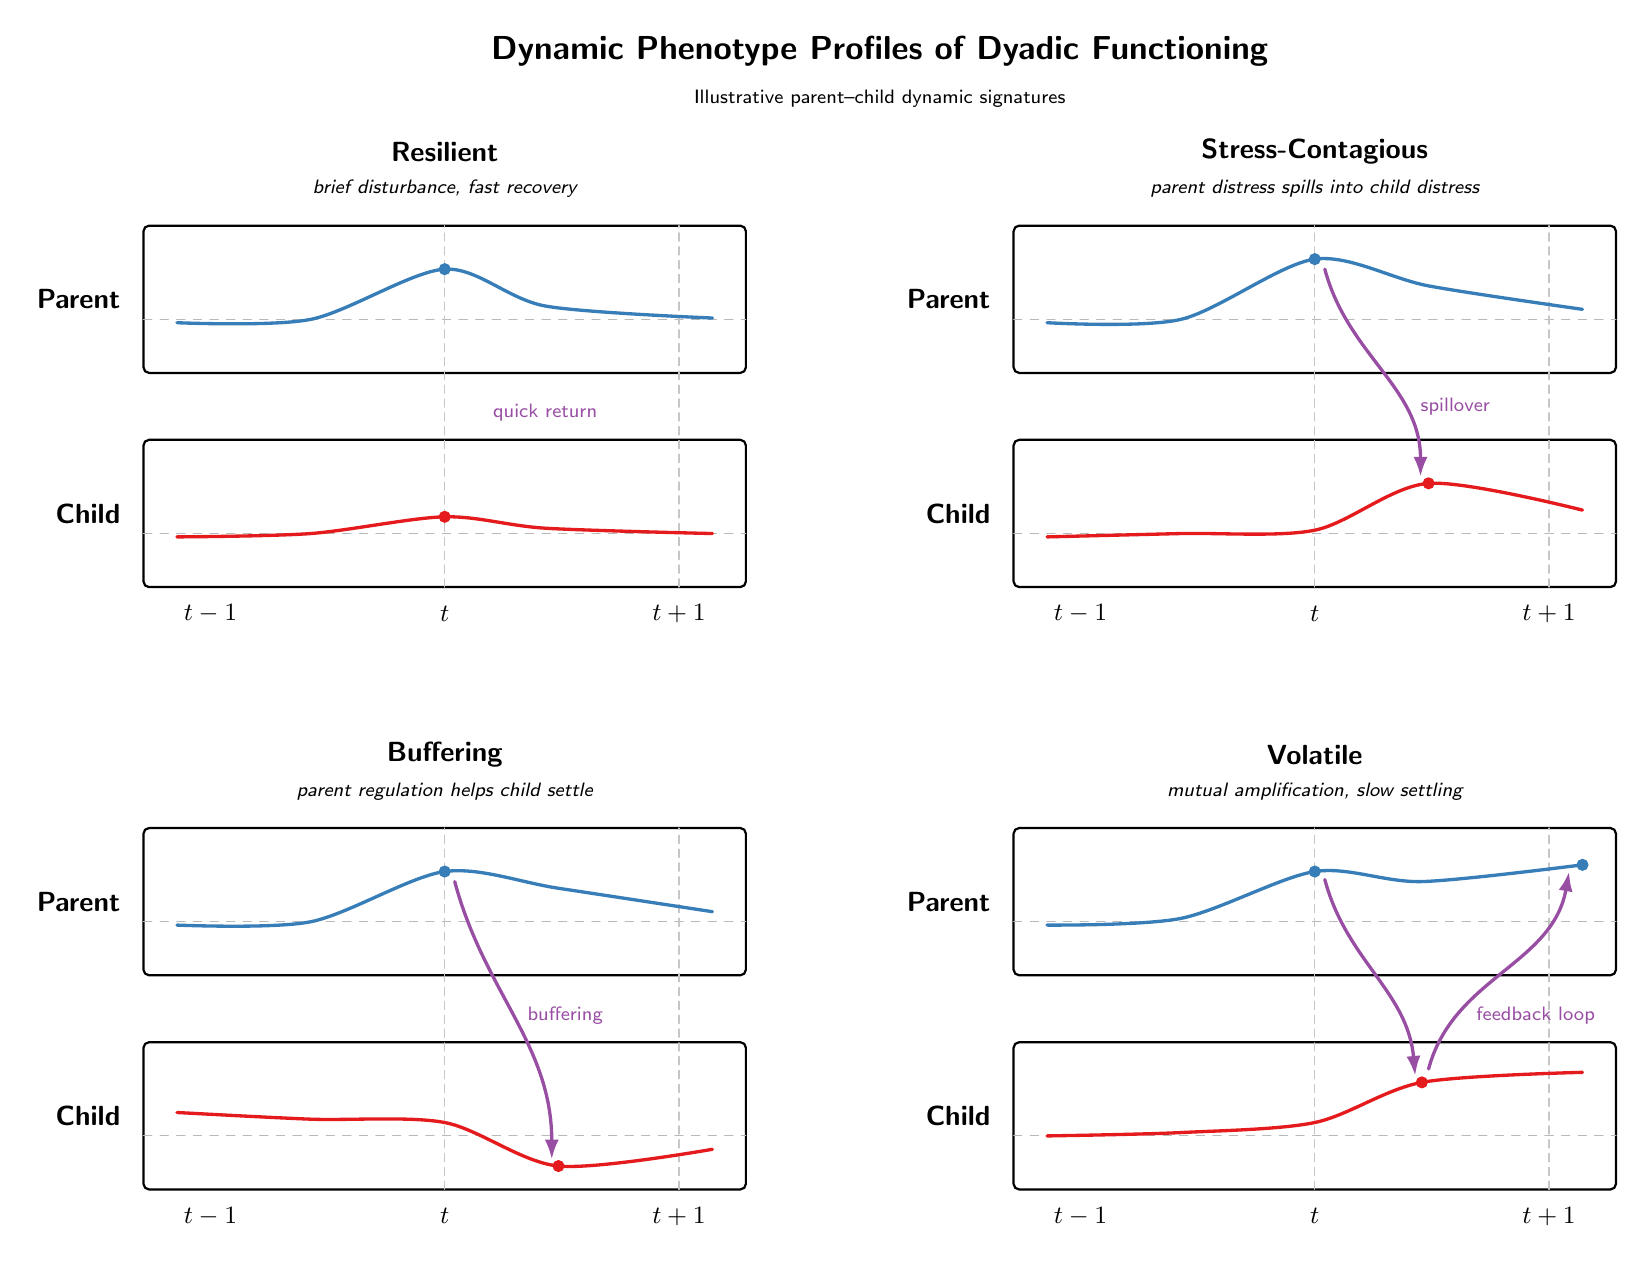
\begin{tikzpicture}[
		x=0.85cm,
		y=0.85cm,
		>=Latex,
		line cap=round,
		line join=round,
		panelbox/.style={thick,rounded corners=2pt},
		baseline/.style={dashed,gray!55},
		guide/.style={densely dashed,gray!45},
		note/.style={font=\scriptsize,align=center},
		phenotitle/.style={font=\bfseries},
		subtitle/.style={font=\scriptsize\itshape,align=center},
		parentline/.style={very thick,draw=myblue},
		childline/.style={very thick,draw=myred},
		parentdot/.style={circle,fill=myblue,draw=myblue,inner sep=1.4pt},
		childdot/.style={circle,fill=myred,draw=myred,inner sep=1.4pt},
		flow/.style={-{Latex[length=2.5mm,width=1.8mm]},very thick,draw=myviolet}
	]
	
	% =========================================================
	% Overall title
	% =========================================================
	\node[font=\bfseries\large] at (11,17.4)
	{Dynamic Phenotype Profiles of Dyadic Functioning};
	
	\node[note] at (11,16.7)
	{Illustrative parent--child dynamic signatures};
	
	% =========================================================
	% PHENOTYPE 1: RESILIENT
	% =========================================================
	\begin{scope}[shift={(0,9)}]
		
		\node[phenotitle] at (4.5,6.9) {Resilient};
		\node[subtitle] at (4.5,6.35) {brief disturbance, fast recovery};
		
		\draw[panelbox] (0,3.6) rectangle (9,5.8);
		\draw[panelbox] (0,0.4) rectangle (9,2.6);
		
		\node[anchor=east,font=\bfseries] at (-0.2,4.7) {Parent};
		\node[anchor=east,font=\bfseries] at (-0.2,1.5) {Child};
		
		\draw[baseline] (0,4.4) -- (9,4.4);
		\draw[baseline] (0,1.2) -- (9,1.2);
		
		\draw[guide] (4.5,0.4) -- (4.5,5.8);
		\draw[guide] (8,0.4) -- (8,5.8);
		
		\node[font=\small] at (1,0) {$t-1$};
		\node[font=\small] at (4.5,0) {$t$};
		\node[font=\small] at (8,0) {$t+1$};
		
		% Parent quick recovery
		\draw[parentline]
		plot[smooth] coordinates {
			(0.5,4.35) (2.5,4.4) (4.5,5.15) (6.0,4.6) (8.5,4.42)
		};
		
		% Child mild bump then recovery
		\draw[childline]
		plot[smooth] coordinates {
			(0.5,1.15) (2.5,1.2) (4.5,1.45) (6.0,1.28) (8.5,1.2)
		};
		
		\node[parentdot] at (4.5,5.15) {};
		\node[childdot] at (4.5,1.45) {};
		
		\node[note,text=myviolet] at (6.0,3.0) {quick return};
		
	\end{scope}
	
	% =========================================================
	% PHENOTYPE 2: STRESS-CONTAGIOUS
	% =========================================================
	\begin{scope}[shift={(13,9)}]
		
		\node[phenotitle] at (4.5,6.9) {Stress-Contagious};
		\node[subtitle] at (4.5,6.35) {parent distress spills into child distress};
		
		\draw[panelbox] (0,3.6) rectangle (9,5.8);
		\draw[panelbox] (0,0.4) rectangle (9,2.6);
		
		\node[anchor=east,font=\bfseries] at (-0.2,4.7) {Parent};
		\node[anchor=east,font=\bfseries] at (-0.2,1.5) {Child};
		
		\draw[baseline] (0,4.4) -- (9,4.4);
		\draw[baseline] (0,1.2) -- (9,1.2);
		
		\draw[guide] (4.5,0.4) -- (4.5,5.8);
		\draw[guide] (8,0.4) -- (8,5.8);
		
		\node[font=\small] at (1,0) {$t-1$};
		\node[font=\small] at (4.5,0) {$t$};
		\node[font=\small] at (8,0) {$t+1$};
		
		\draw[parentline]
		plot[smooth] coordinates {
			(0.5,4.35) (2.5,4.4) (4.5,5.3) (6.2,4.9) (8.5,4.55)
		};
		
		\draw[childline]
		plot[smooth] coordinates {
			(0.5,1.15) (2.5,1.2) (4.5,1.25) (6.2,1.95) (8.5,1.55)
		};
		
		\node[parentdot] (p1) at (4.5,5.3) {};
		\node[childdot] (c1) at (6.2,1.95) {};
		
		\draw[flow] ($(p1)+(0.15,-0.15)$) to[out=-75,in=90] ($(c1)+(-0.12,0.10)$);
		\node[note,text=myviolet] at (6.6,3.1) {spillover};
		
	\end{scope}
	
	% =========================================================
	% PHENOTYPE 3: BUFFERING
	% =========================================================
	\begin{scope}[shift={(0,0)}]
		
		\node[phenotitle] at (4.5,6.9) {Buffering};
		\node[subtitle] at (4.5,6.35) {parent regulation helps child settle};
		
		\draw[panelbox] (0,3.6) rectangle (9,5.8);
		\draw[panelbox] (0,0.4) rectangle (9,2.6);
		
		\node[anchor=east,font=\bfseries] at (-0.2,4.7) {Parent};
		\node[anchor=east,font=\bfseries] at (-0.2,1.5) {Child};
		
		\draw[baseline] (0,4.4) -- (9,4.4);
		\draw[baseline] (0,1.2) -- (9,1.2);
		
		\draw[guide] (4.5,0.4) -- (4.5,5.8);
		\draw[guide] (8,0.4) -- (8,5.8);
		
		\node[font=\small] at (1,0) {$t-1$};
		\node[font=\small] at (4.5,0) {$t$};
		\node[font=\small] at (8,0) {$t+1$};
		
		\draw[parentline]
		plot[smooth] coordinates {
			(0.5,4.35) (2.5,4.4) (4.5,5.15) (6.2,4.9) (8.5,4.55)
		};
		
		\draw[childline]
		plot[smooth] coordinates {
			(0.5,1.55) (2.5,1.45) (4.5,1.4) (6.2,0.75) (8.5,1.0)
		};
		
		\node[parentdot] (p2) at (4.5,5.15) {};
		\node[childdot] (c2) at (6.2,0.75) {};
		
		\draw[flow] ($(p2)+(0.15,-0.15)$) to[out=-75,in=90] ($(c2)+(-0.10,0.10)$);
		\node[note,text=myviolet] at (6.3,3.0) {buffering};
		
	\end{scope}
	
	% =========================================================
	% PHENOTYPE 4: VOLATILE
	% =========================================================
	\begin{scope}[shift={(13,0)}]
		
		\node[phenotitle] at (4.5,6.9) {Volatile};
		\node[subtitle] at (4.5,6.35) {mutual amplification, slow settling};
		
		\draw[panelbox] (0,3.6) rectangle (9,5.8);
		\draw[panelbox] (0,0.4) rectangle (9,2.6);
		
		\node[anchor=east,font=\bfseries] at (-0.2,4.7) {Parent};
		\node[anchor=east,font=\bfseries] at (-0.2,1.5) {Child};
		
		\draw[baseline] (0,4.4) -- (9,4.4);
		\draw[baseline] (0,1.2) -- (9,1.2);
		
		\draw[guide] (4.5,0.4) -- (4.5,5.8);
		\draw[guide] (8,0.4) -- (8,5.8);
		
		\node[font=\small] at (1,0) {$t-1$};
		\node[font=\small] at (4.5,0) {$t$};
		\node[font=\small] at (8,0) {$t+1$};
		
		\draw[parentline]
		plot[smooth] coordinates {
			(0.5,4.35) (2.5,4.45) (4.5,5.15) (6.1,5.0) (8.5,5.25)
		};
		
		\draw[childline]
		plot[smooth] coordinates {
			(0.5,1.2) (2.5,1.25) (4.5,1.4) (6.1,2.0) (8.5,2.15)
		};
		
		\node[parentdot] (p3) at (4.5,5.15) {};
		\node[childdot] (c3) at (6.1,2.0) {};
		\node[parentdot] (p4) at (8.5,5.25) {};
		
		\draw[flow] ($(p3)+(0.15,-0.12)$) to[out=-75,in=95] ($(c3)+(-0.10,0.10)$);
		\draw[flow] ($(c3)+(0.10,0.20)$) to[out=75,in=-100] ($(p4)+(-0.20,-0.10)$);
		
		\node[note,text=myviolet] at (7.8,3.0) {feedback loop};
		
	\end{scope}
	
\end{tikzpicture}

\end{document}
